\begin{frame}
    \titlepage
\end{frame}

{
\setbeamercolor{background canvas}{bg=blue!40!black,fg=blue!10!white}
\setbeamercolor{normal text}{bg=blue!40!black,fg=blue!10!white}
\setbeamercolor{itemize/enumerate body}{fg=white}
\setbeamercolor{itemize/enumerate subbody}{fg=white}
\setbeamercolor{titlelike}{bg=blue!40!black,fg=blue!10!white}
\begin{frame}<1|handout:1>[noframenumbering]{Changelog}
    \begin{itemize}
        \item Corrections made in this version not in first posting:
        \begin{itemize}
        \item 13 Feb 2017: slide 5: {\tt a\textbackslash*} instead of {\tt a\textbackslash}
        \end{itemize}
    \end{itemize}
\end{frame}
}

\section{continuation: virus options}

\begin{frame}{on due dates}
\end{frame}

\begin{frame}{ASM assignment questions?}
\end{frame}

\begin{frame}{last time}
    \begin{itemize}
    \item places to put malicious code
        \begin{itemize}
        \item replace executable
        \item append/prepend
        \item cavities
        \item bootloaders/OS code
        \end{itemize}
    \item started: ways to get code to run
        \begin{itemize}
        \item replace start address
        \item \myemph<2>{replace instructions that are run}
            \begin{itemize}
            \item identify returns/function calls/etc.
            \end{itemize}
        \end{itemize}
    \end{itemize}
\end{frame}

\begin{frame}<3>[label=invokeOptions]{invoking virus code: options}
    \begin{itemize}
    \item boot loader
    \item \myemph<2>{change starting location} 
    \item alternative approaches: ``entry point obscuring''
    \item \myemph<3>{edit code that's going to run anyways}
    \item \myemph<4>{replace a function pointer} (or similar)
    \item \ldots
    \end{itemize}
\end{frame}

\begin{frame}[fragile,label=runAnyways]{run anyways?}
    \begin{itemize}
    \item add code at start of program (Vienna)
    \item return with padding after it:
\begin{Verbatim}[fontsize=\fontsize{10}{11}\selectfont,commandchars=Q\{\}]
  404a01:       c3                      Qtextbf{retq}
  404a02:       0f 1f 40 00             nopl   0x0(%rax)
                Qtextit{replace with}
  404a01:       e9 XX XX XX XX          Qtextbf{jmpq    YYYYYYY}
\end{Verbatim}
    \item any random place in program?
        \begin{itemize}
        \item just not in the \myemph{middle of instruction}
        \end{itemize}
    \end{itemize}
\end{frame}

\begin{frame}[fragile,label=findValidFindFunc2]{recall: finding function calls}
\lstset{language=myasm,style=small}
    \begin{itemize}
    \item e.g. some popular compilers started x86-32 functions with
\begin{lstlisting}
foo:
    push %ebp       // push old frame pointer
    // 0x55
    mov %esp, %ebp  // set frame pointer to stack pointer
    // 0x89 0xec
\end{lstlisting}
    \item use to identify when {\tt e8} ({\tt call} opcode) refers to real function
    \begin{itemize}
    \item (full version: also have some other function start patterns)
    \end{itemize}
    \end{itemize}
\end{frame}



\begin{frame}[fragile,label=stubReplace]{remember stubs?}
\begin{Verbatim}[commandchars=Q\{\},fontsize=\fontsize{8}{9}\selectfont]
0000000000400400 <puts@plt>:
  400400:	ff 25 12 0c 20 00    	jmpq   *0x200c12(%rip) 
                    /* 0x200c12+RIP = _GLOBAL_OFFSET_TABLE_+0x18 */
  400406:	68 00 00 00 00       	pushq  $0x0
  40040b:	e9 e0 ff ff ff       	jmpq   4003f0 <_init+0x28>
    Qtextbf{ replace with: }
  400400:	e8 XX XX XX XX          Qtextbf{jmpq virus_code}
  400405:       90                      nop
  400406:	68 00 00 00 00       	pushq  $0x0
  40040b:	e9 e0 ff ff ff       	jmpq   4003f0 <_init+0x28>
\end{Verbatim}
\begin{itemize}
    \item in known location (particular section of executable)
    \item dynamic linker: just modifies global offset table
\end{itemize}
\end{frame}


\subsection{replacing pointers}

\againframe<4>{invokeOptions}

\begin{frame}[fragile,label=stubsReplacePtr]{stubs again}
\begin{Verbatim}[commandchars=Q\{\},fontsize=\fontsize{8}{9}\selectfont]
0000000000400400 <puts@plt>:
  400400:	ff 25 12 0c 20 00    	jmpq   Qtextbf{*0x200c12(%rip)}
                    /* 0x200c12+RIP = Qtextbf{_GLOBAL_OFFSET_TABLE_+0x18} */
  400406:	68 00 00 00 00       	pushq  $0x0
  40040b:	e9 e0 ff ff ff       	jmpq   4003f0 <_init+0x28>
\end{Verbatim}
\begin{itemize}
\item don't edit stub --- edit initial value of {\tt \_GLOBAL\_OFFSET\_TABLE}
    \begin{itemize}
    \item stored in data section of executable
    \end{itemize}
\item originally: pointer to {\tt 0x400406}; new --- pointer to virus code
\item virus can {\tt jmp} back to {\tt 0x400406} when done
\end{itemize}
\end{frame}

\begin{frame}[fragile,label=relocReplace]{relocations?}
\begin{Verbatim}[commandchars=Q\{\},fontsize=\fontsize{8}{9}\selectfont]
hello.exe:     file format elf64-x86-64

DYNAMIC RELOCATION RECORDS
OFFSET           TYPE              VALUE 
0000000000600ff8 R_X86_64_GLOB_DAT  __gmon_start__
0000000000601018 R_X86_64_JUMP_SLOT  Qtextit{puts@GLIBC_2.2.5}
    Qtextbf{replace with:}
0000000000601018 R_X86_64_JUMP_SLOT  Qtextbf{_start + offset_of_virus}
0000000000601020 R_X86_64_JUMP_SLOT  __libc_start_main@GLIBC_2.2.5
\end{Verbatim}
\begin{itemize}
    \item<1-> tricky --- usually no symbols from executable in dynamic symbol table
        \begin{itemize}
        \item (debugger/disassembler symbols are different tables)
        \item Linux --- need to link with {\tt -rdynamic}
        \end{itemize}
    \item<2-> but\ldots same idea works on shared library itself
\end{itemize}
\end{frame}

\begin{frame}{infecting shared libraries}
\begin{tikzpicture}
    \draw[thick] (0, 0) rectangle (4, -6) coordinate (bottomRight) node[midway] { \tt kernel32.dll };
    \draw[thick,fill=yellow!20] (0, 0) rectangle (4, -0.5) node[midway,font=\small] {header};
    \draw[thick,fill=blue!20] (0, -0.5) rectangle (4, -2.0);
    \node[font=\small,anchor=north] at (2, -0.5) {symbol table};
    \node[anchor=north west,font=\fontsize{9}{10}\selectfont] (GFAName) at (0, -0.9) {
        \tt GetFileAttributesA
    };
    \node[anchor=north west] at (GFAName.south west) {\tt \ldots};
    \draw[-Latex,thick] ([xshift=.5mm]GFAName.east) coordinate (startArrowA) -- ([xshift=.5cm]GFAName.west -| bottomRight) |- (3, -5);
    \fill[black] (startArrowA) circle[radius=.5mm];

    \draw[line width=2mm,-Latex,black!60] (4.6, -3) -- (6.9, -3);
    \begin{scope}[xshift=7cm]
    \draw[thick] (0, 0) rectangle (4, -6) coordinate (bottomRight) node[midway] { \tt kernel32.dll };
    \draw[thick,fill=yellow!20] (0, 0) rectangle (4, -0.5) node[midway,font=\small] {header};
    \draw[thick,fill=blue!20] (0, -0.5) rectangle (4, -2.0);
    \node[font=\small,anchor=north] at (2, -0.5) {symbol table};
    \draw[thick,fill=red!20] (0, -6) rectangle (4, -7) node[midway,font=\small] {virus code};
    \node[anchor=north west,font=\fontsize{9}{10}\selectfont] (GFANameB) at (0, -0.9) {
        \tt GetFileAttributesA
    };
    \node[anchor=north west] at (GFANameB.south west) {\tt \ldots};
    \draw[-Latex,very thick,red] ([xshift=.5mm]GFANameB.east) coordinate (startArrowA) -- ([xshift=.5cm]GFANameB.west -| bottomRight) |- (1, -6.2);
    \fill[red] (startArrowA) circle[radius=.5mm];
    \end{scope}
\end{tikzpicture}
\end{frame}

\begin{frame}{TRICKY}
    \begin{itemize}
    \item next assignment: TRICKY
    \item insert ``tricky jump'' to virus code
        \begin{itemize}
        \item replacing ``{\tt ret}'' followed by cavity of {\tt nop}s
        \end{itemize}
    \item submission: program to modify supplied executable
        \begin{itemize}
        \item need not work on any other program
        \item but, question: how you'd modify it to work on other programs
        \end{itemize}
    \end{itemize}
\end{frame}

\begin{frame}<1>[fragile,label=whyChoices]{virus choices?}
\begin{itemize}
\item why don't viruses always append/replace\tikzmark{append}?
\item why don't viruses always change start location\tikzmark{start}?
\item why did I bother talking about all these strategies?
\end{itemize}
\begin{tikzpicture}[overlay,remember picture]
\coordinate (calloutLoc) at ([yshift=-2cm]current page.center);
\begin{visibleenv}<2>
    \node[mycallout=append] at (calloutLoc) {
        head/tail scanning? 
    };
\end{visibleenv}
\begin{visibleenv}<3>
    \node[mycallout=start]  at (calloutLoc){
        check for suspicious starting location?
    };
\end{visibleenv}
\end{tikzpicture}
\end{frame}

\begin{frame}{more on virus strategies}
    \begin{itemize}
    \item after we talk about anti-virus strategies some
    \end{itemize}
\end{frame}

{ % all template changes are local to this group.
    \setbeamertemplate{navigation symbols}{}
    \contourlength{.2mm}
    \begin{frame}[plain]
        \begin{tikzpicture}[remember picture,overlay]
            \node[at=(current page.center)] {
                
\includegraphics[width=\paperwidth]{1600x1200-Tom-Jerry-Chase}
            };
            %\draw[help lines] (0, 0) grid (12, -8);
            \node[cross out,draw,line width=1mm,black,at={(9,-6)},anchor=center,minimum width=6cm,minimum height=1.25cm] {};
            \node[at={(3,-8.25)},anchor=center,font=\Huge\bfseries,
                red!90!black,align=left] {\contour{black}{Anti-\hspace{-.4ex}Virus}};
            \node[at={(6.5,-8.25)},anchor=center,font=\large\bfseries,
                red!90!black,align=left,rotate=30] {\contour{black}{and}};
            \node[at={(8.5,-8.25)},anchor=center,font=\Huge\bfseries,
                red!90!black,align=left] {\contour{black}{Virus}};
        \end{tikzpicture}
     \end{frame}
}

\begin{frame}{anti-malware strategies}
    \begin{itemize}
    \item antivirus goals:
    \begin{itemize}
    \item prevent malware from running
    \item prevent malware from spreading
    \item undo the effects of malware
    \end{itemize}
    \end{itemize}
\end{frame}

\begin{frame}{malware detection}
    \begin{itemize}
    \item important part: detecting malware
    \item simple way:
        \begin{itemize}
        \item have a copy of a malicious execu\tikzmark{exec}table
        \item compare every\tikzmark{every} program to it
        \end{itemize}
    \end{itemize}
    \begin{tikzpicture}[overlay, remember picture]
        \coordinate (overlayLoc) at ([yshift=-1cm]current page.center);
        \begin{visibleenv}<2>
            \node[mycallout=exec,anchor=center] at (overlayLoc) {
                how big? every executable infected with every virus?
            };
        \end{visibleenv}
        \begin{visibleenv}<3>
            \node[mycallout=every,anchor=center] at (overlayLoc) {
                when? how fast?
            };
        \end{visibleenv}
    \end{tikzpicture}
\end{frame}

\section{signature-based detection}

\begin{frame}{malware ``signatures''}
    \begin{itemize}
    \item antivirus vendor have \myemph{signatures} for known malware
    \item many options to represent signatures
    \item thought process: \myemph{signature for Vienna?}
    \vspace{.5cm}
    \item goals: compact, fast to check, reliable
    \end{itemize}
\end{frame}

\begin{frame}[fragile,label=viennaSigs]{exercise: signatures for Vienna}
\lstset{
        style=smaller,
        language=myasm,
        moredelim={**[is][\btHL<2|handout:0>]{~2~}{~end~}},
        moredelim={**[is][\btHL<3|handout:0>]{~3~}{~end~}},
        moredelim={**[is][\btHL<3-4|handout:0>]{~34~}{~end~}},
        moredelim={**[is][\btHL<4|handout:0>]{~4~}{~end~}},
        }
\begin{tabular}{lll}
\begin{lstlisting}
~2~jmp 0x0700~end~
mov $0x9e4e, %si
...
/* app code */
...
~3~push %cx~end~
mov $0x8f9, %si
...
mov $0x0100, %di
mov $3, %cx
rep movsb
...
\end{lstlisting}
&
\begin{lstlisting}
...
add $0x2f9, %cx
mov %si, %di
sub $0x1f7, %di
mov %cx, (%di)
...
mov $0x288, %cx
mov $0x40 %ah
mov $si, $dx
sub $0x1f9, %dx
int 0x21
...
\end{lstlisting}
&
\begin{lstlisting}
pop %cx
xor %ax, %ax
xor %bx, %bx
~4~xor %dx, %dx~end~
~4~mov $0x0100, %di~end~
~4~push %di~end~
~4~xor %di, %di~end~
~34~ret~end~
/* virus data */
\end{lstlisting}
\\
\end{tabular}
\end{frame}

\begin{frame}{simple signature (1)}
    \begin{itemize}
    \item all the code Vienna copies
    \item \ldots{} except changed {\tt mov} to {\tt \%si}
    \vspace{.5cm}
    \item virus doesn't change it to relocate
    \item includes infection code --- definitely malicious
    \end{itemize}
\end{frame}

\begin{frame}{signature generality}
    \begin{itemize}
    \item the Vienna virus was copied a bunch of times
    \item small changes, ``payloads'' added
        \begin{itemize}
        \item print messages, do different malicious things, \ldots
        \end{itemize}
    \item this signature will not detect any variants
    \item can we do better?
    \end{itemize}
\end{frame}

\begin{frame}{simple signature (2)}
    \begin{itemize}
    \item Vienna start code
        \begin{itemize}
        \item weird jump at beginning??
        \end{itemize}
    \item problem: maybe real applications do this?
    \item problem: easy to move jump
    \end{itemize}
\end{frame}

\begin{frame}{simple signature (3)}
    \begin{itemize}
    \item Vienna infection code
        \begin{itemize}
        \item scans directory, finds files
        \end{itemize}
    \item likely to stay the same in variants?
    \item<2> problem: virus writers \myemph{react to antivirus}
    \end{itemize}
\end{frame}

\begin{frame}{simple signature (4)}
    \begin{itemize}
    \item Vienna finish code
        \begin{itemize}
        \item push + ret 
        \end{itemize}
    \item very unusual pattern
    \item probably(?) not in ``real'' programs
    \item real effort to change to something else?
    \item<2> problem: virus writers \myemph{react to antivirus}
    \end{itemize}
\end{frame}


\begin{frame}{making things hard for the mouse}
    \begin{itemize}
    \item don't want \myemph{trivial changes} to break detection
    \item want to detect \myemph{strategies}
        \begin{itemize}
        \item e.g. require changing relocation logic
        \item \ldots not just reordering instructions
        \end{itemize}
    \item goals: compact, fast to check, reliable, \myemph{general?}
    \end{itemize}
\end{frame}

\begin{frame}{signature checking}
    \begin{itemize}
    \item how fast is signature checking?
    \item problem: lots of I/O?
    \item problem: how complicated are signatures?
    \end{itemize}
\end{frame}

\begin{frame}{generic pattern example}
    \begin{itemize}
    \item another possibility: detect writing near {\tt 0x100}
    \item {\tt 0x100} was DOS program entry code  --- no program should do this(?)
    \item problem: how to represent this?
    \begin{itemize}
        \item describe machine code bytes
        \item multiple possibilities
        \end{itemize}
    \end{itemize}
\end{frame}

\begin{frame}{regular expressions}
    \begin{itemize}
    \item one method of representing patterns like this: \\
          regular expressions (regexes)
    \item restricted language allows very fast implementations
        \begin{itemize}
        \item especially when there's a long list of patterns to look for
        \end{itemize}
    \item homework assignment next week
    \end{itemize}
\end{frame}

\begin{frame}{regular expressions: implementations}
    \begin{itemize}
    \item multiple implementations of regular expressions
    \item we will target: flex, a parser generator
    \end{itemize}
\end{frame}

\begin{frame}[fragile,label=simplePat]{simple patterns}
    \begin{itemize}
    \item alphanumeric characters \myemph{match themselves}
    \item {\tt foo}:
        \begin{itemize}
        \item matches exactly {\tt foo} only
        \item does not match {\tt Foo}
        \item does not match \verb*|foo |
        \item does not match {\tt foobar}
        \end{itemize}
    \item backslash might be needed for others
    \item \verb|C\+\+|
        \begin{itemize}
        \item matches exactly {\tt C++} only
        \end{itemize}
    \end{itemize}
\end{frame}

\begin{frame}[fragile,label=meta1]{metachars (1)}
    \begin{itemize}
    \item special ways to match characters
    \vspace{.5cm}
    \item \verb|\n|, \verb|\t|, \verb|\x3C|, \ldots --- work like in C
    \item \verb|[b-fi]| --- {\tt b} or {\tt c} or {\tt d} or {\tt e} or {\tt f} or {\tt i}
    \item \verb|[^b-fi]| --- any character but {\tt b} or {\tt c} or \ldots
    \item {\tt .} --- any character except newline
    \item \verb!(.|\n)! --- any character
    \end{itemize}
\end{frame}

\begin{frame}[fragile,label=meta2]{metachars (2)}
    \begin{itemize}
    \item \verb|a*| --- zero or more as:
        \begin{itemize}
        \item (empty string), {\tt a}, {\tt aa}, {\tt aaa}, \ldots
        \end{itemize}
    \item \verb|a{3,5}| --- three to five as:
        \begin{itemize}
        \item {\tt aaa}, {\tt aaaa}, {\tt aaaaa}
        \end{itemize}
    \item \verb!(abc){3,5}! --- three to five abcs: (``grouping'')
        \begin{itemize}
        \item {\tt abcabcabc}, {\tt abcabcabcabc}, {\tt abcabcabcabcabc}
        \end{itemize}
    \item {\tt ab|cd}
        \begin{itemize}
        \item {\tt ab}, {\tt cd}
        \end{itemize}
    \item \verb!(ab|cd){2}! --- two ab-or-cds:
        \begin{itemize} 
        \item {\tt abab}, {\tt abcd}, {\tt cdab}, {\tt cdcd}
        \end{itemize}
    \end{itemize}
\end{frame}

\begin{frame}[fragile,label=meta3]{metachars (3)}
    \begin{itemize}
    \item \verb|\xAB| --- the byte {\tt 0xAB}
    \item \verb|\x00| --- the byte {\tt 0x00}
        \begin{itemize}
        \item flex is designed for text, handles binary fine
        \end{itemize}
    \item \verb|\n| --- newline (and other C string escapes)
    \end{itemize}
\end{frame}

\begin{frame}[fragile,label=example1]{example regular expressions}
    \begin{itemize}
    \item match words ending with {\tt ing}: \\
        \verb|[a-zA-Z]*ing|
    \item match C {\tt /* ... */} comments: \\
        \verb!/\*([^*]|\*[^/])*\*/!
    \end{itemize}
\end{frame}

\begin{frame}{flex}
    \begin{itemize}
    \item flex is a regular expression matching tool
    \item intended for writing \myemph{parsers}
    \item generates \myemph{C code}
    \item parser function called {\tt yylex}
    \end{itemize}
\end{frame}


\begin{frame}[fragile,label=flexEx]{flex example}
\lstset{style=small,language={}}
\begin{tikzpicture}
\begin{scope}
\tikzset{every node/.style={font=\small,align=left,anchor=north west,inner sep=0mm}}
\node (vars) {
\begin{lstlisting}
        int num_bytes = 0, num_lines = 0;
        int num_foos = 0;
\end{lstlisting}
};
\node (patMacros) at (vars.south west) {
~
};
\node (sepA) at (patMacros.south west) {
\begin{lstlisting}
%%
\end{lstlisting}
};
\node (pats) at (sepA.south west) {
\begin{lstlisting}
foo     { 
          num_bytes += 3;
          num_foos += 1;
        }
.       { num_bytes += 1; }
\n      { num_lines += 1; num_bytes += 1; }
\end{lstlisting}
};
\node (sepB) at (pats.south west) {
\begin{lstlisting}
%%
\end{lstlisting}
};
\node (mainCode) at (sepB.south west) {
\begin{lstlisting}
int main(void) {
    yylex();
    printf("%d bytes, %d lines, %d foos\n",
           num_bytes, num_lines, num_foos);
}
\end{lstlisting}
};
\end{scope}

\tikzset{
    hi/.style={rounded corners,fill=green,opacity=0.3},
    remark/.style={draw,red,very thick,at={([xshift=-3cm]pats.east)},fill=white,align=left},
    remark2/.style={draw,red,very thick,at={([xshift=-3cm,yshift=2cm]pats.east)},fill=white,align=left},
}

\begin{visibleenv}<2>
    \node[hi,fit=(sepA)] {};
    \node[hi,fit=(sepB)] {};
    \node[remark] {three sections};
\end{visibleenv}

\begin{visibleenv}<3>
    \node[hi,fit=(vars)] {};
    \node[remark] {first --- declarations for later \\
                   C code in output file};
\end{visibleenv}

\begin{visibleenv}<4>
    \node[hi,fit=(pats)] {};
    \node[remark2] {patterns, code to run on match \\
                   as parser: return ``token'' here};
\end{visibleenv}

\begin{visibleenv}<5>
    \node[hi,fit=(mainCode)] {};
    \node[remark] {extra code to include};
\end{visibleenv}

\end{tikzpicture}
\end{frame}

\begin{frame}[fragile,label=flexMatched]{flex: matched text}
\lstset{
        style=small,
        language={},
        moredelim={**[is][\btHL<2|handout:0>]{~2~}{~end~}},
        }
\begin{tikzpicture}
\begin{scope}
\tikzset{every node/.style={font=\small,align=left,anchor=north west,inner sep=0mm}}
\node (vars) {
\begin{lstlisting}
\end{lstlisting}
};
\node (patMacros) at (vars.south west) {
~
};
\node (sepA) at (patMacros.south west) {
\begin{lstlisting}
%%
\end{lstlisting}
};
\node (pats) at (sepA.south west) {
\begin{lstlisting}
[aA][a-z]* {
               printf("found a-word '%s'\n",
                      ~2~yytext~end~);
           }
(.|\n)     {} /* default rule: would output text */
\end{lstlisting}
};
\node (sepB) at (pats.south west) {
\begin{lstlisting}
%%
\end{lstlisting}
};
\node (mainCode) at (sepB.south west) {
\begin{lstlisting}
int main(void) {
    yylex();
}
\end{lstlisting}
};
\end{scope}
\tikzset{
    hi/.style={rounded corners,fill=green,opacity=0.3},
    remark/.style={draw,red,very thick,at={([xshift=-4cm,yshift=2cm]pats.east)},fill=white,align=left},
}
\begin{visibleenv}<2>
    \node[remark] {yytext --- text of matched thing};
\end{visibleenv}
\end{tikzpicture}
\end{frame}


\begin{frame}[fragile,label=flexDef]{flex: definitions}
\lstset{
        style=small,
        language={},
        moredelim={**[is][\btHL<2|handout:0>]{@hi2@}{@endhi@}},
        }
\begin{tikzpicture}
\begin{scope}
\tikzset{every node/.style={font=\small,align=left,anchor=north west,inner sep=0mm}}
\node (vars) {
\begin{lstlisting}
\end{lstlisting}
};
\node (patMacros) at (vars.south west) {
\begin{lstlisting}
A        [aA]
LOWERS   [a-z]
ANY      (.|\n)
\end{lstlisting}
};
\node (sepA) at (patMacros.south west) {
\begin{lstlisting}
%%
\end{lstlisting}
};
\node (pats) at (sepA.south west) {
\begin{lstlisting}
{A}{LOWERS}* {
                printf("found a-word '%s'\n",
                       yytext);
             }
{ANY}        {} /* default rule would
                   output text */
\end{lstlisting}
};
\node (sepB) at (pats.south west) {
\begin{lstlisting}
%%
\end{lstlisting}
};
\node (mainCode) at (sepB.south west) {
\begin{lstlisting}
int main(void) {
    yylex();
}
\end{lstlisting}
};
\end{scope}
\tikzset{
    hi/.style={rounded corners,fill=green,opacity=0.3},
    remark/.style={draw,red,very thick,at={([xshift=-4cm,yshift=2cm]pats.east)},fill=white,align=left},
}
\begin{visibleenv}<2>
    \node[hi,fit=(patMacros)] {};
    \node[remark] {definitions of common patterns \\ included later};
\end{visibleenv}
\end{tikzpicture}
\end{frame}

\usetikzlibrary{arrows,automata}

\begin{frame}[fragile,label=flexHow]{flex: state machines}
\lstset{
        style=small,
        language={},
        moredelim={**[is][\btHL<2|handout:0>]{@hi2@}{@endhi@}},
        }
\begin{tikzpicture}
\node (flexStuff) {
\begin{lstlisting}
foo     {...}
.       {...}
\n      {...}
\end{lstlisting}
};
\begin{scope}[every node/.style={font=\tt,thick}]
\node[initial, state,below=1cm of flexStuff,font=\normalfont\it] (start) {};
\node[state,right=1cm of start] (f) {f};
\node[state,right=1cm of f] (fo) {fo};
\node[state,right=1cm of fo,accepting] (foo) {foo};
\node[state,below right=2cm of start,accepting] (dot) {.};
\node[state,below=1.5cm of start,accepting] (newline) {\textbackslash{}n};
\end{scope}
\path[-Latex,thick] (start) edge node[above] {\tt f} (f)
                    (f) edge node[above] {\tt o} (fo)
                    (fo) edge node[above] {\tt o} (foo)
                    (start) edge node[sloped,above] {other} (dot)
                    (start) edge node[left] {\textbackslash{}n} (newline);
\begin{visibleenv}<2>
    \path[-Latex,blue,dashed] (f) edge node[right] {(back 1)} (dot);
    \path[-Latex,blue,dashed] (fo) edge[out=-45,in=-30] node[midway, sloped, below] {(back 2)} (dot);
\end{visibleenv}
\end{tikzpicture}

\end{frame}

\begin{frame}[fragile,label=stateMachineMatch]{state machine matching}
\begin{tikzpicture}
\node(matchString) {\large \tt \sout<3->{\myemph<2>{a}}\sout<4->{b}\sout<7->{\myemph<5-6>{f}\myemph<6>{oo}}\myemph<7-8>{f}\myemph<7>{\sout<8>{o}}abffoo};

\begin{scope}[every node/.style={font=\tt,thick}]
\node[initial, state,below=1cm of matchString,font=\normalfont\it
      alt=<2>{red}{}] (start) {};
\node[state,right=1cm of start,alt={<5,7>{red}{}}] (f) {f};
\node[state,right=1cm of f,alt={<6,7>{red}{}}] (fo) {fo};
\node[state,right=1cm of fo,accepting,alt={<6>{red}{}}] (foo) {foo};
\node[state,below right=2cm of start,accepting,alt={<3,8>{red}{}}] (dot) {.};
\node[state,below=1.5cm of start,accepting] (newline) {\textbackslash{}n};
\end{scope}
\path[-Latex,thick] (start) edge[alt=<5-7>{red}{}] node[above] {\tt f} (f)
                    (f) edge node[above,alt=<6>{red}{}] {\tt o} (fo)
                    (fo) edge node[above,alt=<6>{red}{}] {\tt o} (foo)
                    (start) edge node[sloped,above,alt=<3>{red}{}] {other} (dot)
                    (start) edge node[left] {\textbackslash{}n} (newline);
\path[-Latex,blue,dashed] (f) edge node[right] {(back 1)} (dot);
\path[-Latex,blue,dashed,alt=<8>{red,thick}{}] (fo) edge[out=-45,in=-30] node[midway, sloped, below] {(back 2)} (dot);
\end{tikzpicture}
\end{frame}

\begin{frame}[fragile,label=flexStates]{flex states (1)}
\lstset{
        style=small,
        language={},
        moredelim={**[is][\btHL<2|handout:0>]{@hi2@}{@endhi@}},
        }
\begin{tikzpicture}
\begin{scope}
\tikzset{every node/.style={font=\small,align=left,anchor=north west,inner sep=0mm}}
\node (vars) {
\begin{lstlisting}
\end{lstlisting}
};
\node (patMacros) at (vars.south west) {
\begin{lstlisting}
%x str
\end{lstlisting}
};
\node (sepA) at (patMacros.south west) {
\begin{lstlisting}
%%
\end{lstlisting}
};
\node (pats) at (sepA.south west) {
\begin{lstlisting}
\"          { BEGIN(str); }
<str>\"     { BEGIN(INITIAL); }
<str>foo    { printf("foo in string\n"); }
foo         { printf("foo out of string\n"); }
<INITIAL,str>(.|\n) {}
\end{lstlisting}
};
\node (sepB) at (pats.south west) {
\begin{lstlisting}
%%
\end{lstlisting}
};
\node (mainCode) at (sepB.south west) {
\begin{lstlisting}
int main(void) {
    yylex();
}
\end{lstlisting}
};
\end{scope}
\tikzset{
    hi/.style={rounded corners,fill=green,opacity=0.3},
    remark/.style={draw,red,very thick,at={([xshift=-5cm,yshift=-2cm]pats.east)},fill=white,align=left},
}
\begin{visibleenv}<2>
    \node[hi,fit=(patMacros)] {};
    \node[remark] {
        declare ``state'' to track \\
        which state determines what patterns are active \\
        \only<3->{``x'' --- exclusive}
    };
\end{visibleenv}
\end{tikzpicture}
\end{frame}

\begin{frame}[fragile,label=flexStates2]{flex states (2)}
\begin{tikzpicture}
\begin{scope}
\tikzset{every node/.style={font=\small,align=left,anchor=north west,inner sep=0mm}}
\node (vars) {
\begin{lstlisting}
\end{lstlisting}
};
\node (patMacros) at (vars.south west) {
\begin{lstlisting}
%s afterFoo
\end{lstlisting}
};
\node (sepA) at (patMacros.south west) {
\begin{lstlisting}
%%
\end{lstlisting}
};
\node (pats) at (sepA.south west) {
\begin{lstlisting}
<afterFoo>foo    { printf("later foo\n"); }
foo              {
                   printf("first foo\n"); 
                   BEGIN(afterfoo);
                 }
(.|\n)  {}  
\end{lstlisting}
};
\node (sepB) at (pats.south west) {
\begin{lstlisting}
%%
\end{lstlisting}
};
\node (mainCode) at (sepB.south west) {
\begin{lstlisting}
int main(void) {
    yylex();
}
\end{lstlisting}
};
\end{scope}
\tikzset{
    hi/.style={rounded corners,fill=green,opacity=0.3},
    remark/.style={draw,red,very thick,at={([xshift=-4cm,yshift=2cm]pats.east)},fill=white,align=left},
}
\begin{visibleenv}<2>
    \node[hi,fit=(patMacros)] {};
    \node[remark] {
        declare non-exclusive state
    };
\end{visibleenv}
\end{tikzpicture}
\end{frame}

% FIXME: flex initial, etc. state stuff

\begin{frame}{why this?}
    \begin{itemize}
    \item (basically) one pass matching
    \item basically speed of file I/O
    \item handles multiple patterns well
    \item flexible for ``special cases''
    \vspace{.5cm}
    \item<2> real anti-virus: probably custom pattern ``engine''
    \end{itemize}
\end{frame}

\begin{frame}{other flex features}
    \begin{itemize}
    \item escape hatch --- I/O directly from code
    \item including ``unget'' function (match normally instead)
    \item allows extra ad-hoc logic
    \end{itemize}
\end{frame}

\begin{frame}{future flex assignment}
    \begin{itemize}
    \item coming weeks --- will have a flex assignment
    \vspace{.5cm}
    \item give you idea what pattern matching can do
    \item produce pattern for {\tt push \$\ldots; ret}.
    \end{itemize}
\end{frame}

\section{example: known virus code}

\begin{frame}[fragile,label=ViennaPat1]{Vienna patterns (1)}
\lstset{
        style=small,
        language={},
        moredelim={**[is][\btHL<2|handout:0>]{@hi2@}{@endhi@}},
        escapechar=`,
        }
\begin{itemize}
\item simple Vienna patterns:
\end{itemize}
\begin{lstlisting}
/* bytes of fixed part of Vienna sample */
\xFC\x89\xD6\x83\xC6\x81\xc7\x00\x01\x83`\textit{(etc)}` {
        printf("found Vienna code\n");
    }
\end{lstlisting}
\end{frame}


\begin{frame}[fragile,label=ViennaPat2]{Vienna patterns (2)}
\lstset{
        style=small,
        language={},
        moredelim={**[is][\btHL<2|handout:0>]{@hi2@}{@endhi@}},
        escapechar=`,
        }
\begin{itemize}
\item simple Vienna patterns:
\end{itemize}
\begin{lstlisting}
/* Vienna sample with wildcards for
   changing bytes: */
/* push %CX; mov ???, %dx; cld; ... */
\x51\xBA@hi2@(.|\n)(.|\n)@endhi@\xFC\x89`\textit{(etc)}` {
        printf("found Vienna code w/placeholder\n");
    }
/* mov $0x100, %di; push %di; xor %di, %di; ret */
\xBF\x00\x01\x57\x31\xFF\xC3 {
        printf("found Vienna return code\n");
    }
\end{lstlisting}
\end{frame}

\begin{frame}{avoiding sensitivity: virus patterns}
    \begin{itemize}
    \item recall: things viruses \myemph{can't easily change!}
    \item example: 
        \begin{itemize}
        \item inserted jumps to virus codes
        \item code in weird parts of executable file
        \item code that modifies executables
        \item \ldots
        \end{itemize}
    \end{itemize}
\end{frame}

\begin{frame}{generic generalizing}
    \begin{itemize}
    \item take static parts of virus
    \item look for \myemph{distance to match}
    \item e.g. {\tt foobarbaz} is 2 from {\tt fooxaxbaz}
    \item slower than regular-expression-like scanners
    \end{itemize}
\end{frame}

\begin{frame}{pattern cost}
    \begin{itemize}
    \item constructed by hand?
        \begin{itemize}
        \item question: how could we automate?
        \end{itemize}
    \item false positives?
        \begin{itemize}
        \item push + ret really unused?
        \item jmp at beginning?
        \item what about data bytes?
        \item \ldots
        \end{itemize}
    \end{itemize}
\end{frame}

\begin{frame}{after scanning --- disinfection}
    \begin{itemize}
    \item antivirus software wants to \myemph{repair}
    \item requires specialized scanning
        \begin{itemize}
        \item no room for errors
        \item need to identify \myemph{all}
        \item need to find relocated bits of code
        \end{itemize}
    \end{itemize}
\end{frame}

\begin{frame}<1>[label=effScanners]{making scanners efficient}
    \begin{itemize}
    \item \myemph<2>{lots of viruses!}
        \begin{itemize}
        \item huge number of states, tables
        \item copies of every piece of malware pretty large
        \end{itemize}
    \item \myemph<3>{reading files is slow!}
    \end{itemize}
\end{frame}

\againframe<2>{effScanners}

\begin{frame}{handling volume}
    \begin{itemize}
    \item storing signature strings is non-trivial
    \item tens of thousands of states???
    \vspace{.5cm}
    \item observation: fixed strings dominate
    \end{itemize}
\end{frame}

\begin{frame}[fragile,label=fixedScan]{scanning for fixed strings}
\begin{tikzpicture}
\tikzset{
    hideOnAdvance/.style={alt=<3>{opacity=0.2}{}},
    hideOnAdvance4/.style={alt={<3,4>{opacity=0.2}{}}},
    myline/.style={line width=0.7mm,-Latex,blue},
    hiString/.style={draw,blue,ultra thick,inner sep=.5mm},
}
\matrix[tight matrix,
    nodes={text width=.5cm,font=\tt\small}
] (string) {
    12 \& 34 \& 56 \& 78 \& 9A \& BC \& DE \& F0 \& 23 \& 45 \& 67 \& 89 \& AB \& CD \& EF \& 03 \& 45 \& 67 \& \ldots \\
};
\node[hideOnAdvance,hiString,fit=(string-1-2) (string-1-17)] (region) {};

\matrix[tight matrix,at={([yshift=-1cm,xshift=-.5cm]string.south east)},anchor=north east,
    nodes={text depth=.35mm},
    column 1/.style={nodes={font=\ttfamily\scriptsize,text width=6cm,
        alt=<4>{opacity=0.4}{}}},
    column 2/.style={nodes={font=\small\itshape,text width=2.2cm}},
    row 1/.style={nodes={font=\normalfont\small\bfseries}}] (patTable) {
    16-byte ``anchor'' \& malware \\
    204D616C6963696F7573205468696E6720 \& Virus A \\
    34567890ABCDEF023456789ABCDEFG0345 \& Virus B \\
    6120766972757320737472696E679090F2 \& Virus C \\
    \ldots                             \& \ldots \\
};
\draw[myline,hideOnAdvance] ([xshift=-4cm]region.south) |- (patTable-3-1.west);
\begin{visibleenv}<3->
\node[draw,minimum height=1cm,below=1.5cm of patTable,font=\itshape] (fulPat){
    (full pattern for Virus B)
};
\draw[myline,hideOnAdvance] (patTable-3-2.east) -- ++(.5cm,0cm) |- (fulPat.east);
\end{visibleenv}
\begin{visibleenv}<4>
\node[hiString,fit=(string-1-3) (string-1-18)] (regionB) {};
\end{visibleenv}
\begin{visibleenv}<5>
\node[draw,red,line width=.5mm,cross out,fit=(patTable-1-1) (patTable-4-1) (patTable.south west),
    inner sep=0mm] (theCross) {};
\begin{pgfonlayer}{fg}
\begin{visibleenv}<2->
\matrix[tight matrix,anchor=center,row sep=-.1mm,
    nodes={text depth=.35mm,fill=white,draw,thick},
    column 1/.style={nodes={font=\ttfamily\scriptsize,text width=3cm}},
    row 1/.style={nodes={font=\normalfont\small\bfseries}},
] (hashTable) at (theCross.center)
{
    4-byte hash \\
    FC923131 \\
    34598873 \\
    994254A3 \\
    \ldots \\
};
\draw[myline,red] ([xshift=-4cm]region.south) -- ++(0cm,-1cm) node[draw,fill=white] {hash function} |- (hashTable-3-1.west);
\end{visibleenv}
\end{pgfonlayer}
\end{visibleenv}
\end{tikzpicture}
\end{frame}

\begin{frame}{real signatures: ClamAV}
\begin{itemize}
\item ClamAV: open source email scanning software
\item signature types:
    \begin{itemize}
    \item hash of file
    \item hash of contents of segment of executable
        \begin{itemize}
        \item built-in executable, archive file parser
        \end{itemize}
    \item fixed string
    \item basic regular expressions
        \begin{itemize}
        \item wildcards, character classes, alternatives
        \end{itemize}
    \item more complete regular expressions
        \begin{itemize}
        \item including features that need more than state machines
        \end{itemize}
    \item meta-signatures: match if other signatures match
    \item icon image fuzzy-matching
    \end{itemize}
\end{itemize}
\end{frame}

\begin{frame}{the I/O problem}
    \begin{itemize}
    \item scanning still requires reading the whole file
    \item can we do better?
    \end{itemize}
\end{frame}

\begin{frame}{selective scanning}
    \begin{itemize}
    \item check entry point and end only
        \begin{itemize}
        \item a lot less I/O, maybe
        \end{itemize}
    \item check known offsets from entry point
    \item heuristic: is entry point close to end of file?
    \end{itemize}
\end{frame}

\againframe<2>{whyChoices}

\begin{frame}[label=playMouse,fragile]{playing mouse}
    \begin{itemize}
    \item techniques so far:
        \begin{itemize}
        \item \myemph<2>{scan for pattern of constant\tikzmark{constant} part of virus}
        \item \myemph<3>{scan for strings, approx. \tikzmark{fixed}16-bytes long}
        \item \myemph<4>{scan \tikzmark{topBottom}top and bottom}
        \end{itemize}
    \item virus-writer hat: how can you defeat these?
    \end{itemize}
    \begin{tikzpicture}[overlay,remember picture]
        %FIXME
        \coordinate (overlayLoc) at ([yshift=-2cm]current page.center);
        \begin{visibleenv}<2>
        \node [mycallout=constant,align=left,anchor=center] at (overlayLoc) { change some trivial part of virus --- \\  e.g. add nops somewhere };
        \end{visibleenv}
        \begin{visibleenv}<3>
        \node [mycallout=fixed,align=left,anchor=center] at (overlayLoc) { insert nops everywhere; \\ split any big strings };
        \end{visibleenv}
        \begin{visibleenv}<4>
        \node [mycallout=topBottom,align=left,anchor=center] at (overlayLoc) { insert jump in middle \\ keep code out of end of file };
        \end{visibleenv}
    \end{tikzpicture}
\end{frame}

\begin{frame}{playing mouse: preview}
    \begin{itemize}
    \item later: metamorphic/polymorphic viruses
        \begin{itemize}
        \item signature resistent
        \item change every time
        \end{itemize}
    \item anti-analysis techniques
        \begin{itemize}
        \item make reverse engineering harder
        \end{itemize}
    \end{itemize}
\end{frame}

\begin{frame}{playing cat}
    \begin{itemize}
    \item harder to fool ways of detecting malware?
    \item goal: small changes to malware preserve detection
    \item ideal: detect \myemph{new} malware
    \end{itemize}
\end{frame}

\begin{frame}<1>[label=detectNew]{detecting new malware}
    \begin{itemize}
    \item \myemph<2>{look for anomalies}
        \begin{itemize}
        \item patterns of code that real executables ``won't'' have
        \end{itemize}
    \item \myemph<3>{identify bad behavior}
    \end{itemize}
\end{frame}

\begin{frame}{viruses and executable formats}
\begin{tikzpicture}
\tikzset{
    mybox/.style={draw,rectangle,minimum width=10cm,fill=white},
}
\node[mybox] (header) {
    \textbf{header}: machine type, file type, etc.
};
\node[mybox,below=0mm of header,align=center] (pHeader) {
    \textbf{program header}: ``\myemph{segments}'' to load \\
        (also, some other information) \\
    \only<2-3>{\myemph{\textbf{length edited by virus}}}
    \only<4-6>{\myemph{\textbf{new segment added by virus}}}
};
\node[mybox,below=0mm of pHeader,align=center] (seg1) {
    \textbf{segment 1 data}
};
\node[mybox,below=0mm of seg1,align=center] (seg2) {
    \textbf{segment 2 data} \\
    \only<2-3>{\myemph{\textbf{virus code + new entry point?}}}
};
\node[mybox,visible on=<4-6>,below=0mm of seg2,align=center] (seg3) {
    \myemph{\textbf{segment 3 data --- virus segment}}
};
\coordinate (annotate) at ([yshift=-1.5cm]seg2.south);
\tikzset{
    annoBox/.style={draw=red,thick,at=(annotate),font=\small,align=center},
}
\begin{visibleenv}<3,5>
    \node[annoBox] {heuristic 1: is entry point in last segment? \\ (segment usually not code)};
\end{visibleenv}
\begin{visibleenv}<6>
    \node[annoBox] {heuristic 2: did virus mess up header? \\ (e.g. do sizes used by linker but not loader disagree)
                \\ section names disagree with usage?};
\end{visibleenv}
\end{tikzpicture}
\end{frame}

\begin{frame}{defeating entry point checking}
    \begin{itemize}
    \item \myemph<2>{insert jump in normal code section, set as entry-point}
    \item add code to first section instead (perhaps insert new section at beginning)
    \end{itemize}
\begin{tikzpicture}
\tikzset{
    annoBox/.style={draw=red,thick,align=center},
}
    \begin{visibleenv}<2>
    \node[annoBox] {
        ``dynamic'' heuristic: run code in VM, see if switches sections
    };
    \end{visibleenv}
\end{tikzpicture}
\end{frame}

\begin{frame}{heuristics: library calls}
    \begin{itemize}
    \item dynamic linking --- functions called \myemph{by name}
    \item how do viruses add to dynamic linking tables?
        \begin{itemize}
        \item often don't! --- instead dynamically look-up functions
        \item if do --- could mess that up/lots of code
        \end{itemize}
    \end{itemize}

    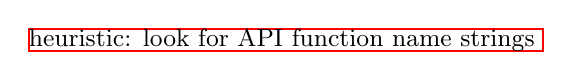
\begin{tikzpicture}
\tikzset{
    annoBox/.style={draw=red,thick,font=\small,align=center},
}
    \node[annoBox] {
        heuristic: look for API function name strings
    };
    \end{tikzpicture}
\end{frame}

\begin{frame}{evading library call checking}
    \begin{itemize}
    \item modify dynamic linking tables
        \begin{itemize}
        \item probably tricky to add new entry
        \end{itemize}
    \item reimplement library call manually
        \begin{itemize}
        \item Windows system calls not well documented, change
        \end{itemize}
    \item \myemph<2>{hide names}
    \end{itemize}
\end{frame}

\begin{frame}{hiding library call names}
    \begin{itemize}
    \item common approach: store \myemph{hash of name}
    \item runtime: read library, scan list of functions for name
    \vspace{.5cm}
    \item bonus: makes analysis harder
    \end{itemize}
\end{frame}

\againframe<3>{detectNew}

\begin{frame}{behavior-based detection}
    \begin{itemize}
    \item things malware does that other programs don't?
    \vspace{.5cm}
    \item<2-> modify system files
    \item<2-> modifying existing executables
    \item<2-> open network connections to lots of random places 
    \item<2-> \ldots
    \vspace{.5cm}
    \item basic idea: run in VM; or monitor all programs
    \end{itemize}
\end{frame}

\begin{frame}{anti-virus: essential or worthless?}
    \begin{itemize}
    \item ungraded homework assignment
    \item watch Hanno B\"ock's talk ``In Search of Evidence-Based IT Security''
    \item a rant mostly about antivirus-like software
    \end{itemize}
\end{frame}


